\section{Android-Client}

In diesem Abschnitt wird die Entwicklung der Android-Bibliothek beschrieben. Zur Entwicklung wurde die plattformübergreifende IDE \emph{IntelliJ Idea}\footnote{IntelliJ Idea: \url{http://www.jetbrains.com/idea/}} verwendet.

Alternativ kann auch die offizielle Anroid \ac{IDE}, \emph{Android Studio}\footnote{Android Studio: \url{http://developer.android.com/sdk/installing/studio.html}}, verwendet werden, welches auf der \emph{Community Edition} von \emph{IntelliJ Idea} basiert, sich zum aktuellen Zeitpunkt jedoch nur in einer \emph{early access preview} verfügbar ist.
Die Projektdateien sind untereinander kompatibel.

Für UML-Diagramme wird die quelloffene, Eclipse basierte, Modellierungssoftware \emph{modelio}\footnote{modelio: \url{http://www.modelio.org/}} genutzt.

Screenshots und Anleitungen beziehen sich diesbezüglich auf diese Software. Konfigurationen und Einstellungen können sich zu anderen IDEs unterscheiden.
Die Quellen zu den Projekten befinden sich im Github-Repository im Unterordner \texttt{client}.

Als Hilfen für die Implementierung dienten hauptsächlich das Buch \citetitle{android4} von \citeauthor*{android4}, sowie einige Tutorials von \citeauthor*{androidvogella}\footnote{\citeauthor*{androidvogella}: \url{http://www.vogella.com/}}.
Außerdem wurden für spezielle Probleme Lösungen Antworten und Quelltextauszüge von der Frage-Antwort-Website StackOverflow\footnote{StackOverflow: \url{http://stackoverflow.com/}} genutzt.
Diese sind in den Kommentaren in den Quelltexten der jeweiligen Klassen vermerkt.


\subsection{Ziele der Implementierung}
Bei der Konzeption und Entwicklung der Android Bibliothek wurden mehrere Ziele verfolgt.
Das Hauptziel ist die Erstellung einer Bibliothek, die sich leicht in Anwendungen integrieren lässt und die Funktionen aufwändiger Mobilgeräte-\ac{UX}-Testaufbauten mit externen Kameras, Mikrofonen etc. ersetzt.
Dazu sollen die technischen Möglichkeiten moderner Endgeräte genutzt werden.
Viele Smartphones und Tablets verfügen über eine Frontkamera für Videotelefonie, ein eingebautes, hochempfindliches, Mikrofon für (Freisprech-)Telefonie und Mehrkernprozessoren für Multitasking.

Diese Eigenschaften sollen genutzt werden um klobige Testaufbauten zu ersetzen. Deren Funktionalität besteht meist aus dem Aufzeichnen von Mimik und Sprache der Testperson, sowie Inhalt des Bildschirms und Interaktion mit dem Endgerät bzw. der Applikation.
Unter der Prämisse, dass moderne Smartphones und Tablets die nötigen Hard- und Softwarevoraussetzungen erfüllen soll nun eine Software Lösung implementiert werden, um die zuvor genannten Funktionen abzubilden.


\subsection{Verwendete Bibliotheken von Drittanbietern}
Neben dem offiziellen Android SDK \footnote{API Level 19, Android 4.4.2} werden die folgenden externe Bibliotheken eingesetzt:
\begin{description}
	\item[Android Asynchronous Http Client\footnote{Android Asynchronous Http Client: \url{http://loopj.com/android-async-http/}}] 
	Ein Callback-basierter HTTP Client, aufbauend auf Apache HTTP\footnote{\url{http://hc.apache.org/httpcomponents-client-ga/}} Bibliotheken. Diese quelloffene Android Bibliothek bietet Klassen und Methoden für asynchrone HTTP Aufrufe und wird auch in großen Projekten wie \emph{Instagram} oder \emph{Pinterest} eingesetzt. Die zusätzliche Abstraktionsschicht übernimmt die Fehlerbehandlung, wiederholte Verbindungsversuche und das übertragen von großen Datenmengen auf einfach anzuwendende Weise. Das Projekt unter der Apache License, Version 2.0\footnote{\url{http://www.apache.org/licenses/LICENSE-2.0}}, veröffentlicht und kann unter deren Bedingungen frei genutzt werden.
	\item[Google GSON\footnote{Google GSON: \url{https://code.google.com/p/google-gson/}}]
	Der Datenabruf vom Server erfolgt mittels \ac{JSON}-Objekte im HTML Body. Um diese Objekte schnell und einfach in Java Objekte umzuwandeln bietet GSON entsprechende Klassen an, die das Implementieren von eigenen Parsern etc. überflüssig macht.
	Die quelloffenen, universell einsetzbare, Java Bibliothek wird ebenfalls unter der Apache License, Version 2.0 veröffentlicht.
%	\item[Android Support Library\footnote{\url{http://developer.android.com/tools/support-library/index.html}}]
%	Diese zusätzliche, nicht im Android SDK enthaltene, Bibliothek bietet zahlreiche zusätzliche Klassen an, die nicht Bestandteil des offiziellen SDK sind, jedoch nützliche Erweiterungen. Z.B. gibt es Klassen für die applikationsinterne Kommunikation und zusätzliche \ac{UI}-Elemente und Layouts.
%	Diese Bibliothek steht unter der \emph{Creative Commons Attribution 2.5}\footnote{http://creativecommons.org/licenses/by/2.5/} Lizenz und kann unter deren Bedingungen verwendet werden.
\end{description}


\subsection{Bibliotheksmodul}
Zur Entwicklung der Bibliothek wurden zwei Projekte verwendet - Einmal das Projekt für die Bibliothek selbst und weiterhin ein Android-Projekt zum Testen der Funktionen während der Entwicklung. 

Ziel der Entwicklung ist ein funktionsfähiger Prototyp, in welchem geplante Kernfunktionen implementiert sind.
Die vorliegende Implementierung ist als \emph{Proof of Concept} anzusehen und weder vollständig, noch frei von Fehlern und Bugs.

\subsubsection{Testapplikation}
Für die Entwicklung und das Testen der Bibliothek wird eine Applikation benötigt in die diese eingebunden wird.
Dazu wurde eine kleine Testapplikation entwickelt, die verschiedene \ac{UI}-Elemente enthält.
Diese setzen sich aus einigen häufig verwendeten, gewöhnlichen \ac{UI}-Klassen des Android SDK zusammen \footnote{\url{http://developer.android.com/design/building-blocks/index.html}}:
\begin{itemize}
	\item Activities
	\item Views
	\item Fragments
	\item Buttons
	\item Dialoge
	\item Toasts.
\end{itemize}
Anfangs bestand die Testapplikation aus einer einzigen Activity und wurde im Verlauf des Projekts erweitert.
In Anhang \ref{anhang:test_app_screens} sind die einzelnen Activities der Testapplikation dargestellt.
Ausgehend von der Haupt-Activity (grau umrandet) lässt sich eine Liste (blau), ein Dialog (grün), ein WebView (violet) und eine einfache Activtiy bestehend aus zwei Fragmenten (rot) öffnen.
Dies reizt zwar nicht die gesamte Palette an Gestaltungsmöglichkeiten aus, reicht jedoch für erste Tests aus.

\subsubsection{Monolithischer Wrapper}
Um die Benutzung zu vereinfachen soll sich die Bibliothek möglichst einfach in neue und bestehende Anwendungen integrieren lassen.
Dies wird u.a. dadurch erreicht, dass Aufrufe nur an eine einzige Klasse gerichtet werden.
Die dahinter liegenden Klassen werden im Sinne des \emph{Facade}-Entwurfsmusters \cite[vgl.][40\psq]{designpattern} \enquote{abgeschirmt}.
Die Klasse \texttt{Hipsterbility} bildet die Schnittstelle zu der Applikation, welche die Bibliothek verwendet.
Diese Art der Abstraktion soll die Benutzung vereinfachen, da nur mit einer einzigen Klasse interagiert werden muss. 
Dies reduziert die Anzahl der Methodenaufrufe auf ein Minimum, wie im Beispiel angedeutet (siehe Listing \ref{list_hipsterbility_client_init}).

%TODO: ggf überarbeiten, falls nötig
\begin{lstlisting}[label=list_hipsterbility_client_init,language=Java, caption=Beispiel für Initialisierung der Android-Bibliothek]
// Singleton Instanz holen und aktuelle Activity uebergeben
Hipsterbility.getInstance().enableTesting(this);

// Module aktivieren
Hipsterbility.MODULE.VIDEO.enabled 	= true; 	// Frontkamera
Hipsterbility.MODULE.AUDIO.enabled 	= true;		// Mikrofon
Hipsterbility.MODULE.SCREEN.enabled = true;		// Bildschirminhalt
\end{lstlisting}

Funktionen können über die öffentliche, verschachtelte statische Aufzählung \texttt{MODULE} in der Klasse \texttt{Hipsterbility} gesteuert.
Jedes Element hat eine boolsche Variable \texttt{enabled}.
Hat diese den Wert \texttt{true}, wird die entsprechende Funktion aktiviert.
Die aktivierten Funktionen entscheiden in ihrer Kombination, welche konkrete Implementierung genutzt wird (siehe Abschnitt \ref{sec_module}).

\subsection{Module zur Datenerfassung \label{sec:module}}
Primärziel der Android Bibliothek ist das Sammeln von Daten, die bei der Interaktion mit der zu testenden Anwendung anfallen.
Angelehnt an gängige Testmethoden (siehe Abschnitt \ref{sec:testmethoden}) wird ein beispielhafter Testaufbau mit folgenden Elementen abgebildet:
\begin{enumerate}
	\item Aufnahme des Gesichts der Testperson durch die Frontkamera des Geräts.
	\item Mitschnitt von verbalen Äußerungen mittels des integrierten Mikrofons.
	\item Abgreifen des Bildschirminhalts mit Visualisierung von Benutzereingaben.
\end{enumerate}

Abbildung \ref{pic:modules_class_diagram} zeigt einige Klassen im Paket \texttt{modules}.
Um die Implementierung der einzelnen \enquote{Module} zu vereinheitlichen gibt es ein Interface \texttt{CaptureModule}, welches die benötigten Methodensignaturen enthält und von den \texttt{*Module} Klassen realisiert wird.
Die einzelnen Klassen sind als statische Singletons \cite[vgl.][21\psq]{designpattern} implementiert.
Besonders bei Klassen mit exklusivem Hardwarezugriff (\texttt{CameraCaptureModule, AudioCaptureModule}) wird so verhindert, dass mehrere Objekte erstellt werden, was zu Laufzeitfehlern führen könnte.
Um die Methodenaufrufe 
\begin{wrapfigure}[20]{l}{0.5\textwidth}
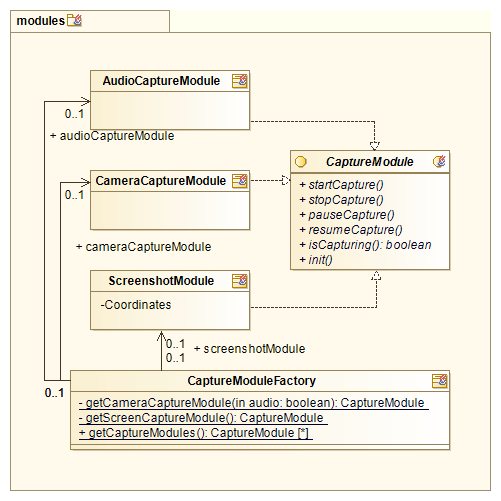
\includegraphics[width=\linewidth]{img/modules_Class_diagram}
\caption{Klassendiagramm des Pakets \mbox{\texttt{modules}}.}
\label{pic:modules_class_diagram}
\end{wrapfigure}


\subsubsection{Frontkamera und Mikrofon}
Bei der Auswertung von Usability-Tests kann die Mimik der Testperson zur Interpretation beitragen.
Außerdem kann durch das Kamerabild gesehen werden, ob die Testperson sich auf die gestellte Aufgabe konzentriert oder abgelenkt ist.
Dies ist von Bedeutung, wenn der Zeitfaktor bei der Auswertung berücksichtigt wird.
Neben dem Kamerabild werden Sprache und Umgebungsgeräusche mit dem integrierten Mikrofon aufgezeichnet.
Einerseits können so unbewusste Aussagen aufgezeichnet und bewertet werden, andererseits erlaubt dies den Einsatz von \emph{Thinking Aloud Tests}, bei denen die Testperson gezielt subjektive Eindrücke verbal äußert.  %TODO: Belege suchen

Die Herausforderung bei der Implementierung stellt sich durch Beschränkungen des Android Betriebssystems.
Dieses sieht vor, dass bei der Aufnahme von Videos und Fotos mit der Kamera eine Vorschau auf dem Bildschirm dargestellt wird.
Dieser soll jedoch vollständig der zu testenden Anwendung zur Verfügung stehen.
Die Lösung besteht darin einen \texttt{SurvaceView} zu erstellen, welcher als System Overlay über allen anderen Bildschirmelementen gezeichnet wird. 
Dieser wird mit einem transparenten Pixelformat versehen, auf 1x1 Pixel verkleinert und in die obere linke Bildschirmecke verschoben.

Somit wird eine, für den Benutzer nicht sichtbare, Vorschau erstellt und die Aufzeichnung kann über die vom System bereitgestellten Klassen erfolgen.


\subsubsection{Bildschirminhalt mit Root-Zugriff}
Mit Root-Zugriff ist das erstellen einzelner Screenshots mit wenigen Zeilen Quelltext möglich, wie in Listing \ref{listing:screenshot_root} dargestellt.

\begin{lstlisting}[label=listing:screenshot_root,language=Java, caption=Screenshot Aufnahme mit Root-Zugriff]
sh = Runtime.getRuntime().exec("su", null, null); // Superuser Rechte holen
OutputStream os = sh.getOutputStream();
os.write("/system/bin/screencap -p /sdcard/outputfile.png"); // Screenshot erstellen
os.flush(); // Schreibpuffer leeren 
os.close(); // und schliessen
sh.waitFor(); // Auf Beendigung der o.g. Befehle warten
\end{lstlisting}

Ab Android 4 wird ein natives Kommandozeilenprogramm \texttt{screencap} mitgeliefert.
Dieses erlaubt das Erstellen von Screenshots, indem direkt der \emph{FrameBuffer} des Systems ausgelesen wird (siehe Quelltext zu \texttt{screencap}\footnote{screencap Quelltext: \url{https://github.com/android/platform_frameworks_base/blob/master/cmds/screencap/screencap.cpp}}).
Der Parameter \texttt{-p} gibt an, dass das Ausgabeformat \texttt{PNG} sein soll. 
Optional kann noch die Nummer des Displays nach dem optionalen Parameter \texttt{-d} angegeben werden.
Am Ende des Aufrufs steht der Pfad der Ausgabedatei, im Beispiel \texttt{/sdcard/outputfile.png}. 

Das \emph{Rooting} des Android Betriebssystems wird von diesem selbst nicht verhindert, jedoch muss ggf. der Bootloader entsperrt werden, was zu einer Löschung der Gerätedaten aus Sicherheitsgründen führen kann. 
Neben den Vorteilen, die \emph{Rooting} bietet, wie z.B. erweitertes Debugging oder vollständige Backups, so hat es einige Nachteile oder ist teilweise nicht mit einfachen Möglichkeiten erreichbar \cite[vgl.][]{androidsecurity}.
Um das \emph{Rooting} oder die Installation von alternativen Betriebssystemen oder Versionen zu verhindern verschlüsseln einige Hersteller die Bootloader ihrer Geräte \cite[vgl.][6\psq]{androiddataintegrity}.

Der Vollzugriff auf das Dateisystem und das Betriebssystem kann jedoch auch zu Sicherheitsproblemen führen und daher z.B. in Unternehmen für betrieblich genutzte Geräte untersagt werden.
Demnach kann nicht davon ausgegangen werden, dass nicht immer ein Root-Zugriff möglich ist.

\subsubsection{Bildschirminhalt ohne Root-Zugriff}
Da ohne Root-Zugriff nicht auf die nativen Anwendungen zugegriffen werden kann, wurde eine alternative Lösung entwickelt.
Die Bibliothek läuft bei der Ausführung der Applikation in deren Kontext und im selben Prozess.
Dadurch ist es möglich auf die Activities der Applikation zuzugreifen.

In Listing \ref{listing:screenshot} ist dargestellt, wie ein Bild von einer Activity erstellt wird.
Der direkte Zugriff auf den FrameBuffer oder andere Stationen der Ausgabekette ist nicht möglich, daher wird der Bildschirminhalt \enquote{nachgezeichnet}.
Mit dieser Implementierung werden allerdings nur grafische Elemente der Anwendung erfasst, ein Zugriff auf die Statusleiste, Navigationsleiste oder andere Anwendungen ist so nicht möglich.

\begin{lstlisting}[label=listing:screenshot,language=Java, caption=Screenshot Aufnahme ohne Root-Zugriff]
Display display = activity.getWindowManager().getDefaultDisplay();
Point size = new Point();
display.getSize(size);
// RootView holen
View view = activity.getWindow().getDecorView().getRootView();
// Bitmap und Canvas erstellen
Bitmap bitmap = Bitmap.createBitmap(size.x, size.y, Bitmap.Config.ARGB_4444);
Canvas canvas = new Canvas(bitmap);
// Theme holen und anwenden
final Resources.Theme theme = activity.getTheme();
final TypedArray ta = theme.obtainStyledAttributes(new int[]{android.R.attr.windowBackground});
final int res = ta.getResourceId(0, 0);
final Drawable background = activity.getResources().getDrawable(res);
// Hintergrund zeichnen
background.draw(canvas);
// Views zeichnen
view.draw(canvas);
// Bild komprimieren und ins Dateisystem schreiben
FileOutputStream fos = new FileOutputStream("/sdcard/screenshot.png"));
bitmap.compress(Bitmap.CompressFormat.PNG, 90, fos);
fos.flush();
fos.close();
\end{lstlisting}

Das erstellen eines Bildes der Anwendung verläuft in mehreren Schritten.
Über die \texttt{Activity} kann auf den \texttt{WindowManager} und auf das Standarddisplayobjekt zugegriffen werden, um die Bildschirmgröße zu bestimmen.
Danach wird der \texttt{RootView}, der alle anderen grafischen Elemente enthält als Referenz zwischengespeichert.
Zum erstellen des Bildes wird ein \texttt{Bitmap} in Bildschirmgröße erstellt um anschließend ein \texttt{Canvas} Objekt zu erzeugen, auf dem grafische Elemente gezeichnet werden können.
Darauf werden nun nacheinander, beginnend mit dem Hintergrund, die grafischen Elemente gezeichnet.

Abschließend wird das Bild komprimiert und in eine Datei geschrieben.

\subsubsection{Visualisieren von Benutzereingaben}

\subsection{Weitere Funktionen und Ausblick}

\subsection{Einbinden der Bibliothek in eigene Anwendungen}


\subsection{Benutzeroberfläche und Integration in Android Applikationen}


\subsubsection{Dynamisches Einbinden - Pre-Dexing}

Beim Pre-Dexing können mehrere Android-Projekte zu einem Projekt hinzugefügt werden. 
%TODO: updating

Da die Bibliothek neueste Funktionen des Android-Betriebssystems verwendet, muss auf dem  Gerät zur Kompilierung einer Anwendung aktuelle Build-Tools der Android-SDK vorliegen.
Im Falle der Bibliothek ist dies API-Level 19. Offenbar hat sich hier ein Bug eingeschlichen und es ist unter der Version 19.0 kein Pre-Dexing möglich.
Dies wurde allerdings bereits behoben. Es sei gesagt, dass mindestens die Version 19.0.1 verwendet werden muss um Pre-Dexing durchführen zu können.
%TODO: update, wichtig? Screenshot? 

\subsubsection{Statisches Einbinden als JAR-Archiv}

\subsection{Bekannte Einschränkungen}
Der gegenwärtige Stand der Bibliothek enthält einige Einschränkungen bei der Nutzung. 
Einerseits sind Video- und Screenshotaufnahme, basierend auf nativen Funktionen mit Root-Zugriff zwar implementiert und getestet, allerdings nicht vollständig in den Gesamtablauf eingebunden und können entsprechend nicht beim Testen von Applikationen genutzt werden.
%TODO: Entfernen wenn doch noch implementiert
Auch der Wechsel von Activities wird aktuell noch nicht voll unterstützt.
Wenn keine Activity der Testanwendung mehr im Vordergrund ist wird zwar die Aufnahme nach einem Timeout gestoppt, beim Wechsel in eine andere Activty der Testapplikation wird diese nicht weiter aufgezeichnet.
Nur die Video- und Audioaufzeichnung im Hintergrund wird fortgesetzt, der Bildschirminhalt wird nicht weiter aufgezeichnet.

Weiterhin werden -- nicht bildschirmfüllende -- Elemente wie Dialoge, Benachrichtigungen und Toasts bei der Bildschirmaufzeichnung nicht erfasst, da i.d.R. über Systemdienste erstellt werden.

Auch der Ablauf von Tasks und Todos lässt sich im aktuellen Stand nicht nachverfolgen.
Außerdem hat die Testperson aktuell keine Möglichkeit sich -- nach dem Start einer Session -- noch einmal die Aufgabenstellung anzusehen.

Eine weitere Hürde stellt der Orientierungswechsel des Geräts während der Datenerfassung dar, da die Orientierung des Kamerabildes nur beim starten der Aufnahme bestimmt wird.
Das erstellen von Screenshots funktioniert zwar weiterhin, allerdings nicht das native Screen Recording.
Bei diesem würde ein Teil des Bildbereichs abgeschnitten und schwarze Balken eingefügt.
 
 
\subsection{Ausblick und Weiterentwicklung}

\subsubsection{Application Lifecycle}
Neben den Interaktionen des Benutzers mit einzelnen Activities oder Bildschirmelementen kann auch eine Auswertung des Lebenszyklus der Applikation und enthaltener Activities Aufschlüsse liefern.
So kann beispielsweise durch das (automatische) statistische Auswerten von entsprechenden Logdateien analysiert werden, in welcher Häufigkeit und Reihenfolge Activities aufgerufen werden, oder ob einzelne gar nicht gestartet werden, weil z.B. ein Button nicht funktioniert oder Testpersonen die Funktion nicht finden.

\subsubsection{Protokollierung von Benutzereingaben}
Auch wenn Benutzereingaben auf den Aufnahmen vom Bildschirminhalt visualisiert werden, kann eine zusätzliche Protokollierung in maschinenlesbaren weitere (automatisierte) Analysemöglichkeiten bieten.
Anhand von statistischen Analysen kann z.B. herausgefunden werden, dass Testpersonen Reaktionen auf Gesten erwarten, die nicht implementiert wurden.
Zusätzlich können Zeitabstände zwischen einzelnen Eingaben ausgewertet und interpretiert werden, um herauszufinden wie leicht verständlich Benutzeroberflächen durch Testpersonen wahrgenommen werden.

\subsection{Benutzeroberfläche und Interaktion}
Bisher werden Testpersonen nur wenig Möglichkeiten geboten Aufgaben nachzuverfolgen oder nachzuschlagen.
Beim Start einer Session werden diese Angezeigt, können aktuell, im Verlauf der Datenerfassung, allerdings nicht noch einmal aufgerufen werden.
Auch das Layout und Design der Benutzeroberfläche können weiter verbessert werden.
Einige Symbole dienen nur als Platzhalter können gegen passendere ersetzt werden.
Bisher wurden Layout und Design einzig für Smartphones optimiert, sie funktionieren schlecht auch auf Tablets, da nur wenige Informationen auf einen deutlich größeren Bildschirm dargestellt werden.

\subsection{Sicherheit}
Die Kommunikation mit dem Server verläuft unverschlüsselt mittels \ac{HTTP}-Methoden.
Auch Benutzername und Passwort werden aktuell unverschlüsselt im Klartext übertragen und können einfach Mitgelesen werden.
Die Speicherung des Passworts auf dem Endgerät erfolgt durch das Android Pereferences Framework in unverschlüsselten Textdateien und kann mit Root-Zugriff leicht ausgelesen werden.  
Um die Kommunikation sicherer zu gestalten sollte die Kommunikation verschlüsselt werden, z.B. mittels \ac{SSL} bzw. \ac{TLS}, da das Android Betriebssystem Bibliotheken für diese Verfahren mitbringt.
Zur sichereren Speicherung von Benutzername und Passwort könnte z.B. die Android interne Kontenverwaltung genutzt werden.